
\chapter{Ugeopgave 5-7}

Denne ugeopgaves form�l var at implementere og forst�
\emph{radiosity}-metoden.

\paragraph{Bem�rk}
\label{sec:bemark}

Dele af den eksekverbare fil (del 5 og 6) til denne opgave virker ikke
p� de gamle maskiner i VR-baren. De virker dog p� de nye. Vi har ikke
kunnet finde grunden til det.

\section{Del 1}
\label{sec:ex5-1}

F�rste opgave er at downloade kildekoden og compile den. Det skulle
vise cornell scenen med uden radiosity. Scenen kan ses p� figur
\ref{figur-5-1-1}.

\begin{figure}[htbp]
  \centering
  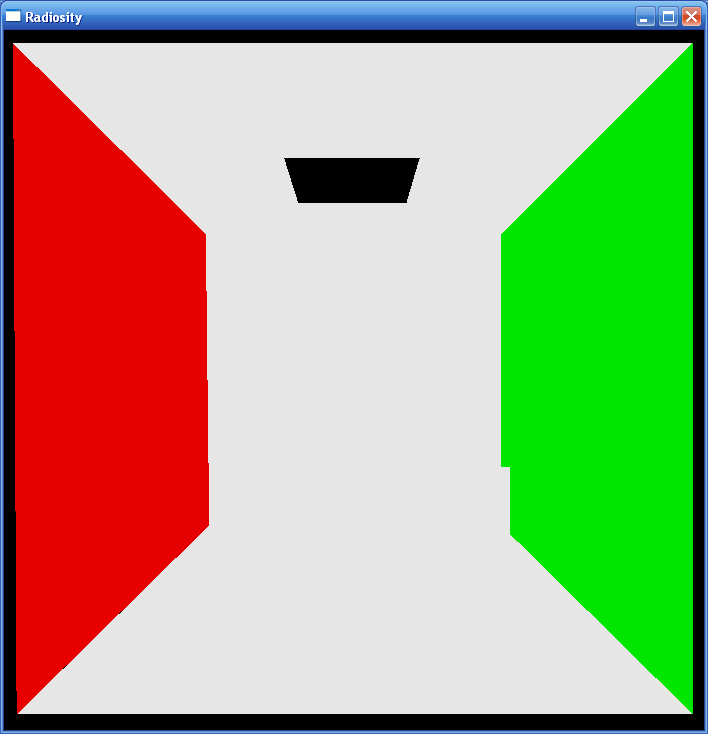
\includegraphics[width=8cm]{screenshots/ex5/1.png}
  \caption{hej}
  \label{figur-5-1-1}
\end{figure}

\section{Del 2}
\label{sec:ex5-2}

Dern�st skal scenen \textit{meshes}. P� figur \ref{figur-5-2-1} kan vi
se scenen delt op i mindre stykker med brug af mesher biblioteket.

\begin{figure}[htbp]
  \centering
  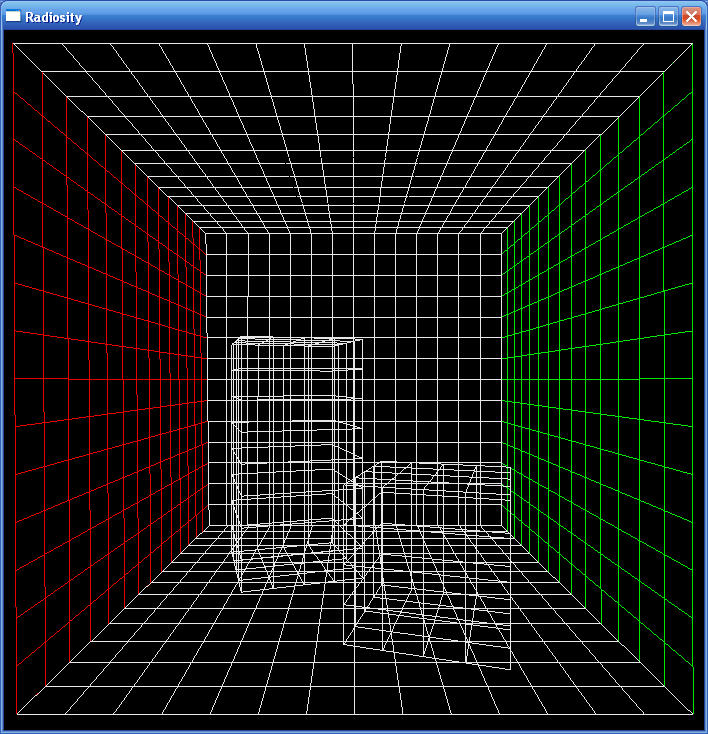
\includegraphics[width=8cm]{screenshots/ex5/2.png}
  \caption{}
  \label{figur-5-2-1}
\end{figure}

\section{Del 3}
\label{sec:ex5-3}

I 3. del af opgaven skal vi lave \textit{progressive refinement}. Det
kr�ver at vi implementerer f�lgende funktioner som skal bruger i hver
itteration af main loopet:

\begin{itemize}
\item En funktion der finder den \textit{patch} med st�rst energi.
\item En funktion der udregner \textit{form factors} mellem en
  \textit{patch} og alle de andre \textit{patches}. Dette g�res
  analytisk.
\item En funktion der distribuerer energi fra en \textit{patch} til
  alle andre \textit{patches}
\item En funktion der beregner farven af alle \textit{patches}.
\end{itemize}

Resultatet kan ses p� figur \ref{figur-5-3-1}. Billedet viser tydeligt
firkanter, men dette bliver bedre n�r vi har lavet opgave 4.

Funktionerne ville vi lave i \texttt{ProgRef.cpp} men da der var nogle
problemer med linking har vi v�ret n�dsaget til at flytte nogle af
funktionerne op i headeren \texttt{ProgRef.h}.

\begin{figure}[htbp]
  \centering
  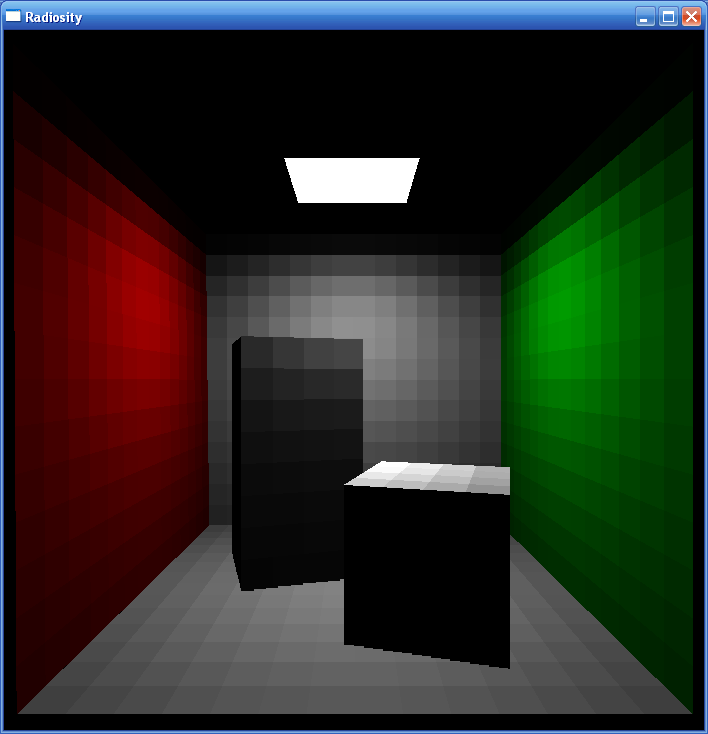
\includegraphics[width=8cm]{screenshots/ex5/3.png}
  \caption{}
  \label{figur-5-3-1}
\end{figure}

\section{Del 4}
\label{sec:ex5-4}

Som n�vn tidligere skal opgave 4 arbejde p� at g�re billedets
farveskift glattere. Vi implementerer derfor \textit{vertex radiosity}
som kaldes \textit{nodal-averages}. Resultatet kan ses af figur
\ref{figur-5-4-1}


\begin{figure}[htbp]
  \centering
  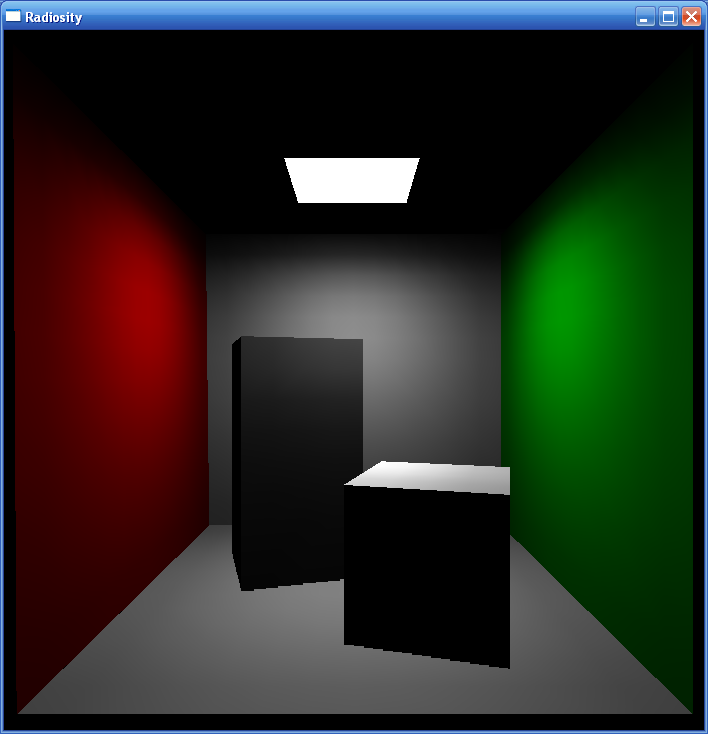
\includegraphics[width=8cm]{screenshots/ex5/4.png}
  \caption{}
  \label{figur-5-4-1}
\end{figure}

\section{Del 5}
\label{sec:ex5-5}

Nu vil vi gerne bruge \texttt{hemicube} metoden istedet for at beregne
\textit{form factors} annalytisk. Derfor anvender vi
\texttt{hemicube.h}. Nu har billedet f�et skygger, modsat
tidligere. Da vi hele tiden har anvendt scenen med kasserne i skifter
vi ikke scene, men det er tydeligt at se forskellen.

I figur \ref{figur-5-5-1} og \ref{figur-5-5-2} ser vi scenen med
skygger med og uden \textit{nodal-averaging}.

\begin{figure}[htbp]
  \centering
  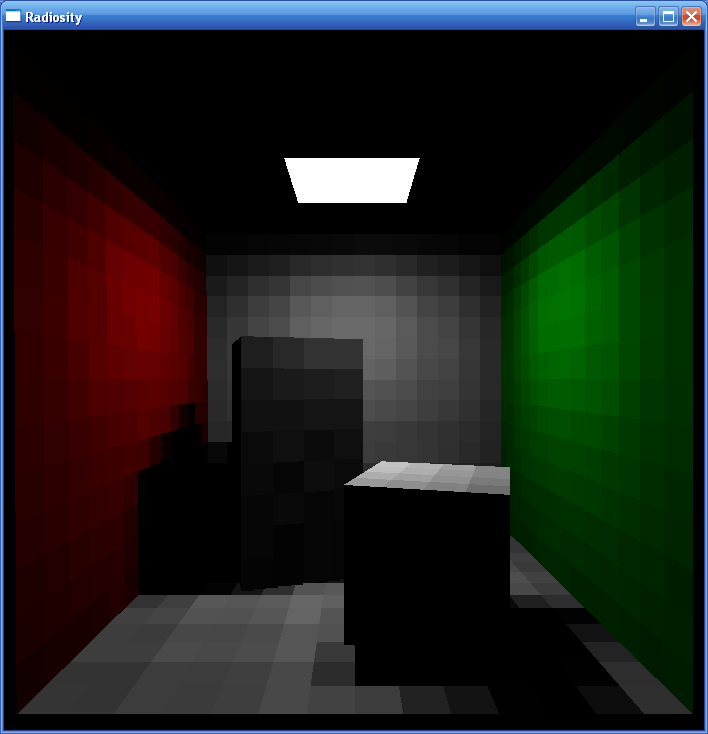
\includegraphics[width=8cm]{screenshots/ex5/5a.png}
  \caption{}
  \label{figur-5-5-1}
\end{figure}

\begin{figure}[htbp]
  \centering
  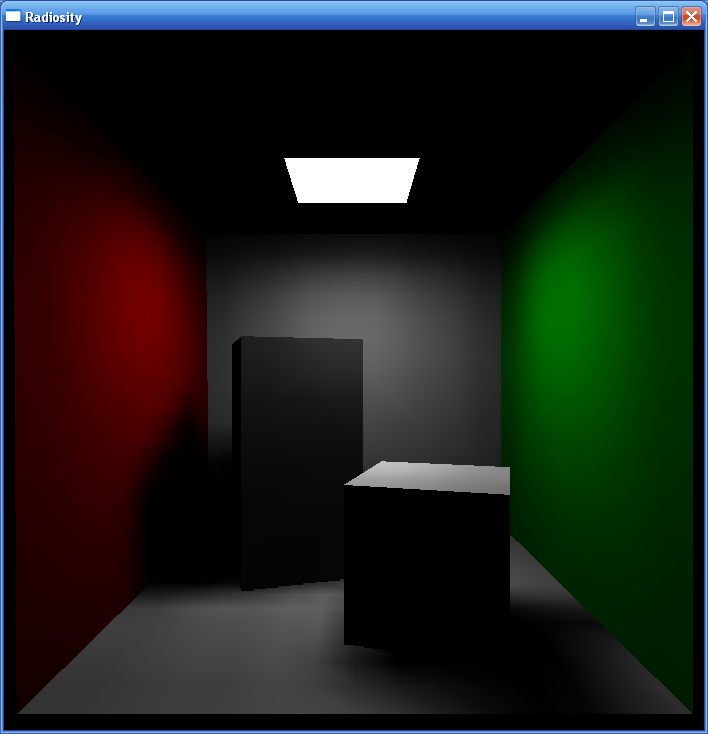
\includegraphics[width=8cm]{screenshots/ex5/5b.png}
  \caption{}
  \label{figur-5-5-2}
\end{figure}

\section{Del 6}
\label{sec:ex5-6}

\textit{What is the effect of changing the subdivision level of the
  light source?}

Et lavt niveau vil resultere i \textit{patches} f�r et meget
\texttt{unshot radiosity} som langsomt konvergerer mod nul og derfor
for�jer tiden det tager at rendere. Der vil ogs� opst�
\textit{aliasing} problemer omkring lyskilden og kanten af
skyggerne. Et for h�jt niveau �del�gger farve \textit{bleeding} og
noget af skyggerne.

\textit{What happens when the size of the hemicube is changed? Why
  does it happen? What can be done to avoid this problem?}

I figur \ref{figur-5-6-1} og \ref{figur-5-6-1} kan vi se hvad der sker
n�r \texttt{hemicuben} er hhv. ekstremt stor og ekstremt lille.

Der opst�r fejl fordi der antages at \textit{patches} projicerer
pr�cist over p� et heltal pixels. Dette er sj�ldent tilf�ldet.

Man kan s�tte opl�sningen af hemicuben op, men det betyder ogs� at
alle der skal regnes langt mere.

\begin{figure}[htbp]
  \centering
  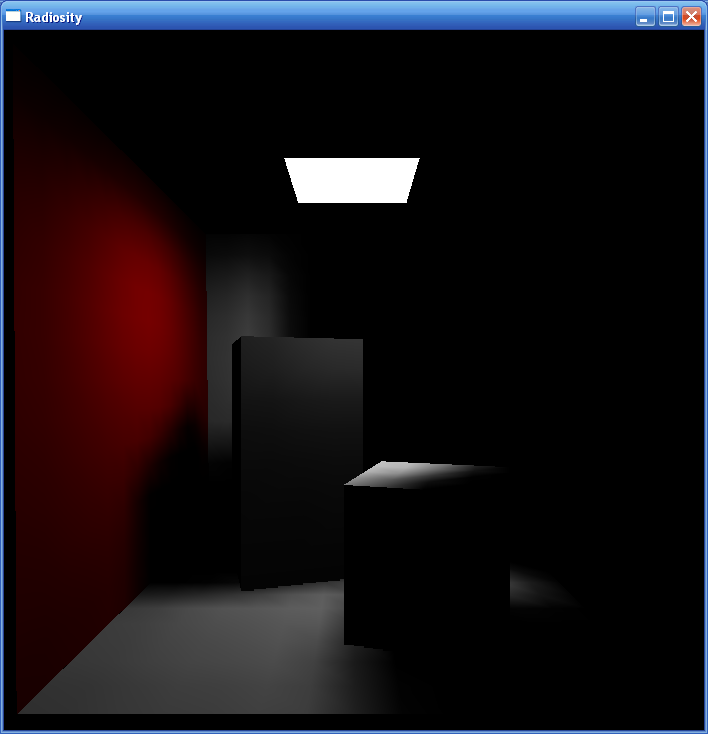
\includegraphics[width=8cm]{screenshots/ex5/6b1.png}
  \caption{}
  \label{figur-5-6-1}
\end{figure}
\begin{figure}[htbp]
  \centering
  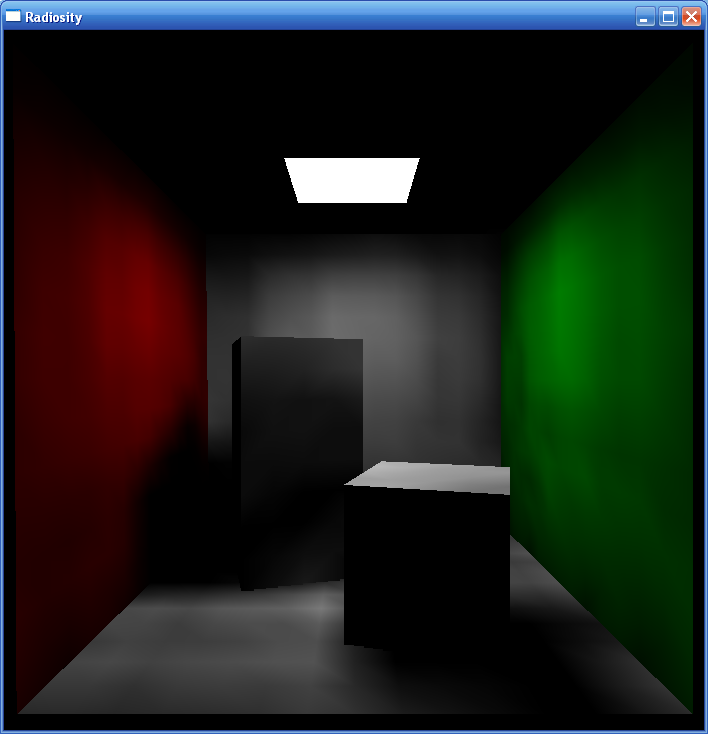
\includegraphics[width=8cm]{screenshots/ex5/6b2.png}
  \caption{}
  \label{figur-5-6-2}
\end{figure}

\textit{What effect can be captured using radiosity, that can not be
  captured using ray tracing?}

\texttt{Radiosity} kan vise diffuse \textit{interreflections}, som
bla. kan ses ved farvernes \texttt{bleed}, i mods�tning til ray
tracing. \texttt{Radiosity} kan h�ndtere LD*E hvor ray tracing bruger
LD?S*E.

%%% Local Variables: 
%%% mode: latex
%%% TeX-master: "report_main"
%%% End: 
